\chapter{Diseño del proyecto}

En este capítulo se trataran los temas relacionados con la fase de diseño del proyecto, es decir, con el estudio previo que se ha realizado de todos los componentes que se encuentran involucrados en él. En esta agrupación se ve envuelta, por ejemplo, la propia vivienda y su composición estructural, ya que es necesario conocer, entre otros, el espacio físico con que se cuenta para colocar los mecanismos y dispositivos situados en los cuadros eléctricos y domóticos, las dimensiones de las habitaciones para establecer que dispositivos cumplirán correctamente sus funciones o cuales requerirán de una mayor inversión en sus capacidades como puede ser el caso de los sensores de movimiento o los sistemas de aerotermia; e incluso conocer los materiales de paredes y techo para no aportarles una carga superior, tanto de peso como temperatura, humedad o cualquier otra magnitud, que no pudiesen aceptar a la hora de instalar y albergar máquinas en su interior, sin sufrir ningún tipo de daño.\\\\
Este estudio tomará especial relevancia una vez que el diseño y el desarrollo hayan concluido, y comience la fase de instalación y volcado de las programaciones, donde los elementos deberán ser colocados en sus respectivos puestos y comenzar a funcionar según se les ha indicado en sus programaciones. Esto se debe a que, en este punto, sin la validación adecuada del diseño previo, podrían presentarse graves problemas que no harían más que encarecer y alargar temporalmente el proyecto, lo que lo alejaría de la meta final de que el cliente se encuentre satisfecho con el resultado de la domotización de su vivienda, a la par de resultar lo más económicamente viable para la empresa.

\section{Elección de componentes}

A continuación, se detalla una lista con los múltiples dispositivos y módulos domóticos que han sido utilizados para desarrollar la solución final diseñada y la funcionalidad que les ha sido otorgada. En esta lista únicamente aparecerán los elementos incluidos en el cuadro eléctrico de domótica y los mecanismos domóticos de la instalación, quedando excluidos, por tanto, los efectores y actuadores puramente eléctricos así como su cuadro, por no encontrarse dentro de las competencias de diseño del sistema.

\subsection{Actuadores} Estos elementos se encargan de ejecutar las acciones solicitadas desde el controlador sobre los diferentes elementos domóticos de la vivienda a los que se encuentra conectado. Existen diversas clases de actuadores que se clasifican en función de la aplicación que vayan a desarrollar. En este proyecto se utilizarán los siguientes:

\begin{itemize}
\item \textbf{Dimmers:} 
	\begin{itemize}
	\item\underline{Descripción:} actuador regulador KNX de 4 elementos.
	\item \underline{Características:} este tipo de actuador permite el control de la regulación del elemento que se encuentra conectado a su salida mediante el uso de dispositivos TRIAC y DIAC. Cuenta con modo de accionamiento manual para modo de prueba, además de protección contra marcha en vacío, cortocircuito y sobretemperatura. 
	\item \underline{Funcionalidad:} la aplicación que ejecutan es la de regulación de la intensidad de la iluminación de algunas de las lámparas de la vivienda.\\ [0,15 cm]
		\begin{figure}[H]
		\centering
		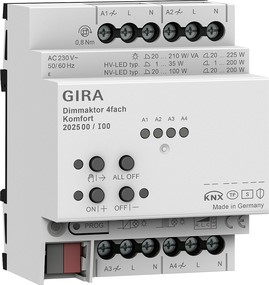
\includegraphics[width=0.35\textwidth]{figures/actuador_dimmer.jpg}   
		\caption{Actuador tipo dimmer}
		\label{fig:actuador_dimmer}
		\end{figure}
	\end{itemize} 


\item \textbf{Binario + persiana:} 
	\begin{itemize}
	\item\underline{Descripción:} actuador de conmutación de 24 elementos / control 12 persianas.
	\item \underline{Características:} este módulo combina la funcionalidad de dos tipos de actuadores diferentes, y permite el control tanto de elementos ON/OFF como de persianas, atendiendo a la funcionalidad con la que se programen sus salidas. Cuenta con modo de accionamiento manual para modo de prueba.
	\item \underline{Funcionalidad:} algunas de sus salidas serán utilizadas para el control de apertura de una ventana y el despliegue de una pantalla de proyección. El resto servirán para el control binario del resto de luces de la casa y de algunas de las tomas de corriente que se han decidido “domotizar”. Otras funcionalidades puntuales de tipo binario que tienen sus salidas son las de accionamiento del timbre, de la sirena de alarma, el control de la cerradura de la vivienda, la velocidad del recuperador, el encendido de la caldera y las electroválvulas de agua y gas.
	\begin{figure}[H]
	\centering
	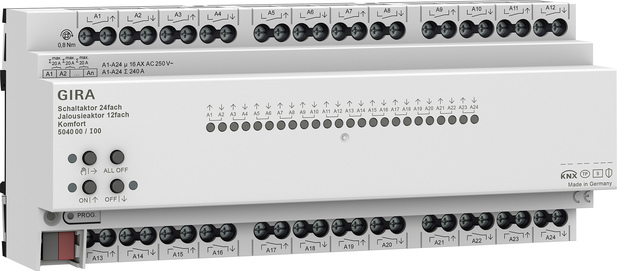
\includegraphics[width=0.55\textwidth]{figures/actuador_binario.png}   
	\caption{Actuador tipo binario/persiana}
	\label{fig:actuador_binario}
	\end{figure}
	\end{itemize} 

\item \textbf{Rejilla + zonificación:} 
	\begin{itemize}
	\item\underline{Descripción:} actuador de control sobre 8 rejillas + 2 unidades de aire acondicionado.
	\item \underline{Características:} esta clase de actuador combina la capacidad de control de la apertura de una rejilla con la de gestión de diferentes temperaturas mediante módulos lógicos. . Cuenta con modo de accionamiento manual para modo de prueba, además de indicadores visuales de movimiento de rejillas mediante LEDs.
	\item \underline{Funcionalidad:} gracias a sus características, nos permite conectarlo con los termostatos distribuidos por la casa y hacer un control por zonas de la distribución del sistema de aerotermia de los fancoils, activando y adecuando la velocidad de sus ventiladores en función de la demanda.
	\begin{figure}[H]
	\centering
	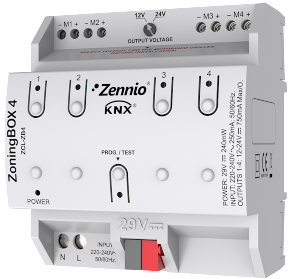
\includegraphics[width=0.35\textwidth]{figures/actuador_rejilla.png}   
	\caption{Actuador tipo zonificación}
	\label{fig:actuador_rejilla}
	\end{figure}
	\end{itemize} 

\item \textbf{Accionamiento térmico:} 
	\begin{itemize}
	\item\underline{Descripción:} actuador de calefacción de 6 elementos.
	\item \underline{Características:} permite la actuación de accionamientos térmicos integrado con un regulador de temperatura ambiente. Incluye la opción del conexionado en cascada de los actuadores.
	\item \underline{Funcionalidad:} las salidas de este módulo irán conectadas a las válvulas de regulación de los entramados del suelo radiante para regular su apertura, así como a la caldera de la vivienda, indicando los momentos en los que esta debe ser activada en función de la demanda de temperatura gestionada por los termostatos. \\ [0,15 cm]
	\begin{figure}[H]
	\centering
	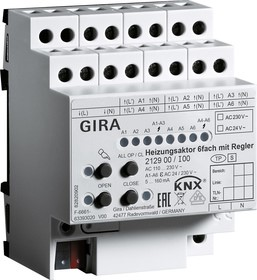
\includegraphics[width=0.35\textwidth]{figures/actuador_termico.jpg}   
	\caption{Actuador tipo térmico}
	\label{fig:actuador_termico}
	\end{figure}
	\end{itemize} 
\end{itemize} 

\subsection{Sensores}

\begin{itemize}
\item \textbf{CO\textsubscript{2}:} 
	\begin{itemize}
	\item\underline{Descripción:} sensor CO\textsubscript{2} con regulador de humedad y temperatura KNX.
	\item \underline{Características:} supervisión del valor de partículas de \textsubscript{2} y de humedad en el ambiente. Alarma de punto de rocío para prevenir la formación de moho en sistemas de refrigeración. Posee dos entradas binarias para la conexión de contactos sin tensión. El sensor de \textsubscript{2} permite ajustar cuatro niveles límites diferentes.
	\item \underline{Funcionalidad:} la funcionalidad con la que ha sido programado es la de, mediante la actuación de tres niveles de partículas de \textsubscript{2}, activar los tres niveles de velocidad del ventilador del recuperador en consecuencia.
	\begin{figure}[H]
	\centering
	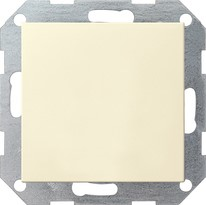
\includegraphics[width=0.30\textwidth]{figures/sensor_co2.jpg}   
	\caption{Sensor de CO\textsubscript{2}}
	\label{fig:sensor_co2}
	\end{figure}
	\end{itemize} 


\item \textbf{Movimiento:} 
	\begin{itemize}
	\item\underline{Descripción:} detector de movimiento de superficie de 2,2 m.
	\item \underline{Características:} configurable para la detección de movimiento o para la monitorización del con capacidad de cuantificar la luminosidad de la estancia para realizar un apagado de la iluminación al superar un umbral configurable. Permite la configuración de un bloque de función para realizar las siguientes funciones: conmutación, función para escaleras, transmisor de valores de regulación, mecanismo auxiliar para escenarios, transmisor de valores de temperatura, transmisor de valores de luminosidad, conmutación de modo de funcionamiento, conmutación con posición forzada.
	\item \underline{Funcionalidad:} serán utilizados para detectar la entrada de personas en determinadas zonas de la vivienda, y en función del modo en que se encuentre el sistema, hará las veces de ON/OFF de las luces de esas zonas o bien hará saltar el sistema de alarma ante intrusiones.
	\begin{figure}[H]
	\centering
	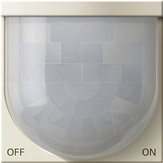
\includegraphics[width=0.25\textwidth]{figures/sensor_movimiento.png}   
	\caption{Sensor de movimiento}
	\label{fig:sensor_movimiento}
	\end{figure}
	\end{itemize} 

\item \textbf{Presencia:} 
	\begin{itemize}
	\item\underline{Descripción:} detector presencia multifunción.
	\item \underline{Características:} posee varios modos de funcionamiento, a saber: detector de presencia, observador de techo o detector de movimiento. La monitorización del entorno se realiza mediante el uso de tres sensores PIR y uno de luminosidad, con lo que se permite utilizar los parámetros de detección de las tres zonas y de luminosidad para hacer un control en intensidad de la iluminación zonal en sintonía con la posibilidad de utilizar las cinco funciones lógicas que permite usar. La funcionalidad de este dispositivo es similar a la del detector de movimiento, pero con los siguientes añadidos: transmisión de valores de regulación, nivel crepuscular ajustable, aplicación de retardos, función de bloqueo y la posibilidad de configuración de límites de luminosidad.
	\item \underline{Funcionalidad:} gracias a su diseño discreto, se instala en el techo del salón con la funcionalidad de controlar la iluminación de la estancia en función de principalmente dos parámetros externos: la presencia de personas y la iluminación exterior, aplicándole un valor de sensibilidad determinado para realizar el ON a partir de la detección de cierta cantidad de luxes.
	\begin{figure}[H]
	\centering
	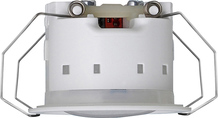
\includegraphics[width=0.35\textwidth]{figures/sensor_presencia.png}   
	\caption{Sensor de presencia}
	\label{fig:sensor_presencia}
	\end{figure}
	\end{itemize}

\item \textbf{Inundación:} 
	\begin{itemize}
	\item\underline{Descripción:} sensor de inundación.
	\item \underline{Características:} es capaz de detectar la presencia de agua en un ambiente.
	\item \underline{Funcionalidad:} será necesario la implementación de un módulo de entradas para poder comunicar los sensores con la instalación KNX de la vivienda.
	\begin{figure}[H]
	\centering
	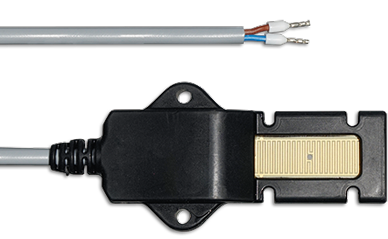
\includegraphics[width=0.35\textwidth]{figures/sensor_inundacion.png}   
	\caption{Sensor de inundación}
	\label{fig:sensor_inundacion}
	\end{figure}
	\end{itemize} 

\item \textbf{Apertura:} 
	\begin{itemize}
	\item\underline{Descripción:} contacto magnético.
	\item \underline{Características:} este sensor consta de dos partes: la primera irá fijada en el marco de la ventana y la segunda, en la propia ventana. Al cerrar la ventana, se cerrará el circuito eléctrico, transmitiendo así un valor por el bus opuesto al que envía al encontrarse abierto.
	\item \underline{Funcionalidad:} su misión será la de ofrecer al sistema información acerca de si las ventanas de la casa se encuentran abiertas o cerradas.
	\begin{figure}[H]
	\centering
	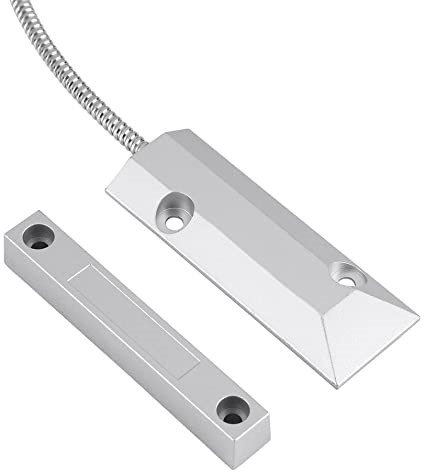
\includegraphics[width=0.35\textwidth]{figures/sensor_apertura.png}   
	\caption{Sensor de apertura}
	\label{fig:sensor_apertura}
	\end{figure}
	\end{itemize} 

\item \textbf{Humo:} 
	\begin{itemize}
	\item\underline{Descripción:} combinación de detector de humos y detector térmico.
	\item \underline{Características:} sensor termovelocimétrico alimentado por pilas. Dos señales acústicas de alarma distintas para cada uno tipos de detección con posibilidad de atenuarse durante la fase de pruebas.
	\item \underline{Funcionalidad:} su objetivo es el de detectar de situaciones anómalas y potencialmente peligrosas relacionadas con los incendios y dar aviso de ello a los usuarios que se encuentren en la vivienda. Para poder ser integrados en la instalación KNX, será necesario la implementación de un módulo extra, que será el encargado de comunicar el detector de humos con el sistema de control de la vivienda.
	\begin{figure}[H]
	\centering
	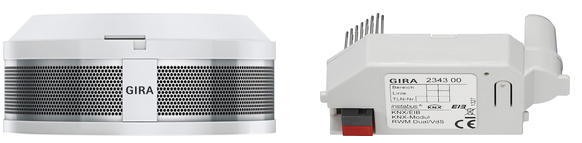
\includegraphics[width=0.75\textwidth]{figures/sensor_humo.png}   
	\caption{Sensor de humo y módulo KNX}
	\label{fig:sensor_humo}
	\end{figure}
	\end{itemize} 
\end{itemize} 

\subsection{Lectores de consumo}

\begin{itemize}
\item \textbf{Electricidad:} 
	\begin{itemize}
	\item\underline{Descripción:} medidor de energía eléctrica para sistemas monofásicos o trifásicos.
	\item \underline{Características:} permite el monitorizar la energía consumida/producida, el coste y las emisiones de \textsubscript{2} asociadas al consumo, la potencia activa y reactiva, el factor de potencia y otra información relacionada con el uso de la energía en la vivienda.
	\item \underline{Funcionalidad:} se monitorizarán la tensión y corriente de fase instantáneos, la potencia activa consumida instantánea y la energía consumida acumulada total y en un periodo de tiempo definido por el usuario, incluyendo la tarifa y sus emisiones de carbono en esos periplos. Se realizarán dichas medidas acoplando un transformador de corriente a cada una de las líneas. 
	\begin{figure}[H]
	\centering
	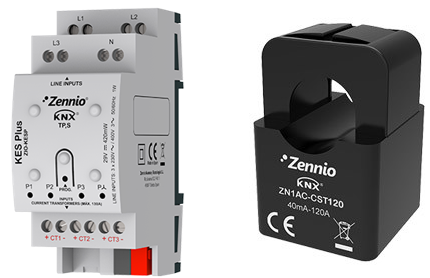
\includegraphics[width=0.55\textwidth]{figures/contador_electricidad.png}   
	\caption{Contador consumo eléctrico y acoplador de línea }
	\label{fig:contador_electricidad}
	\end{figure}
	\end{itemize} 

\item \textbf{Agua y gas:} 
	\begin{itemize}
	\item\underline{Descripción:} interfaz KNX de monitorización de consumo de 4 elementos.
	\item \underline{Características:} permite monitorizar en el bus KNX el consumo eléctrico (energía y potencia), agua y gas mediante el conteo de pulsos SO (salida impulso optoacoplador). Estas medidas pueden visualizarse en consumo instantáneo o acumulado.
	\item \underline{Funcionalidad:} estos módulos serán utilizados para hacer un conteo del consumo acumulado total y desdeuna fecha determinada por el usuario del agua y el gas gastados en la vivienda. Tambien se utilizará su funcionalidad de calculo de tarifas, para que el cliente pueda consultar el gasto en cualquier periplo. Irá conectado directamente a los instrumentos de medida de la vivienda.
	\begin{figure}[H]
	\centering
	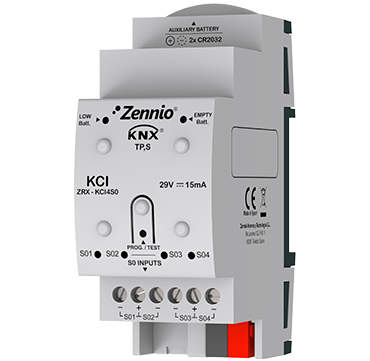
\includegraphics[width=0.35\textwidth]{figures/contador_agua.png}   
	\caption{Contador de consumo de agua y gas}
	\label{fig:contador_agua}
	\end{figure}
	\end{itemize} 
\end{itemize} 

\subsection{Interfaces del usuario}

\begin{itemize}
\item \textbf{Pulsadores domóticos:} 
	\begin{itemize}
	\item\underline{Descripción:} mecanismo acoplador de bus.
	\item \underline{Características:} de la variedad de características que pueden presentar este tipo de elementos, se han escogido los acopladores de bus con pulsación sobre dos elementos con mando de un punto, es decir, pulsadores de dos teclas con posibilidad de pulsarse únicamente en una dirección. 
	\item \underline{Funcionalidad:} control de las lámparas, tanto las binarias como las dimmeables, los enchufes, activación de las velocidades del recuperador, subir y bajar la pantalla del proyector, abrir y cerrar la ventana y activación del timbre.
	\begin{figure}[H]
	\centering
	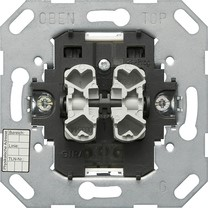
\includegraphics[width=0.30\textwidth]{figures/pulsador.jpg}   
	\caption{Pulsadores domóticos}
	\label{fig:pulsador}
	\end{figure}
	\end{itemize} 

\item \textbf{Termostatos:} 
	\begin{itemize}
	\item\underline{Descripción:} panel táctil capacitivo con display.
	\item \underline{Características:} posee 4 botones con multidisplay de 4 indicadores personalizables. Incluye funcionalidad de termostato, detector de movimiento y 2 puertos de entradas de tipo binario o lectura desde una sonda de temperatura.
	\item \underline{Funcionalidad:} se utilizará su función de termostato para gestionar el sistema de climatización. Desde estos dispositivos se efectuarán las llamadas de demanda tanto al sistema de suelo radiante como a los fancoils, en función de las temperaturas sensadas en cada habitación mediante el uso de una de sus entradas como sonda de temperatura. Uno de los termostatos llevará en su segunda canal de entrada una sonda térmica utilizada para conocer la temperatura exterior a la vivienda. Además, sus botones serán utilizados para las siguientes funciones:
		\begin{itemize}
		\item Los botones en el cuadrante inferior serán utilizados para subir y bajar la temperatura de consigna de la zona en la que se encuentra el termostato.
		\item El botón en el cuadrante superior derecho tendrá la funcionalidad de variar el flujo de aire cedido por los equipos de aire acondicionado. Al ser un único botón, la secuencia que efectuará será cíclica con el siguiente patrón: +, ++, +++, A, +. ++, +++, A, … Siendo A la ejecución del modo automático, que seleccionará la velocidad de los ventiladores en función de la demanda y la ponderación otorgada a cada zona o habitación.
		\item El botón en el cuadrante superior izquierdo servirá para cerrar la rejilla de esa habitación, evitando así el paso del aire de los fancoils.
		\end{itemize} 
	\begin{figure}[H]
	\centering
	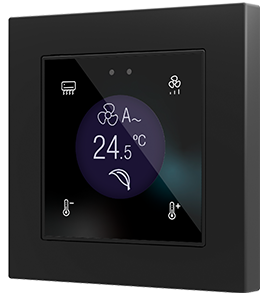
\includegraphics[width=0.37\textwidth]{figures/termostato.png}   
	\caption{Termostato}
	\label{fig:termostato}
	\end{figure}
	\end{itemize} 

\item \textbf{G1:} 
	\begin{itemize}
	\item\underline{Descripción:} es un dispositivo multifunción que permite visualizar y controlar numerosas funciones del edificio relacionadas con el control de los módulos instalados en ellos.
	\item \underline{Características:} posee una infinidad de funcionalidades, por lo que se mencionan únicamente las que poseen un enfoque más focalizado hacia las buscadas en este proyecto: una pantalla táctil con altavoz y micrófono integrados, capacidad de reconocimiento facial y reproducción de vídeo. Es posible personalizar su interfaz de usuario con la posibilidad de utilizar más de 320 iconos de función organizadas por carpetas con un manejo muy intuitivo. 
	\item \underline{Funcionalidad:} será utilizado como monitor y como puesto de control principal de la vivienda, representando la programación volcada sobre el X1. Esta pantalla hará las veces de display para mostrar las cadenas de texto o los datos que puedan resultar de interés para el usuario, como pudieran ser mensajes de alarma, de consumo, de avería o error... 
	\begin{figure}[H]
	\centering
	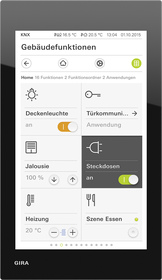
\includegraphics[width=0.25\textwidth]{figures/g1.png}   
	\caption{G1}
	\label{fig:g1}
	\end{figure}
	\end{itemize} 
\end{itemize} 

\subsection{Módulos de entradas}

\begin{itemize}
\item \textbf{Para sensores de apertura:} 
	\begin{itemize}
	\item\underline{Descripción:} entrada binaria KNX de 6 elementos.
	\item \underline{Características:} este módulo posee 6 entradas binarias que transforman sus valores en telegramas KNX. Permite ejecutar dos acciones diferentes por cada flanco, tanto de subida como de bajada, de cada una de las salidas.
	\item \underline{Funcionalidad:} en este proyecto, este mecanismo tendrá como entradas una serie de contactores magnéticos, cuya tarea es la de sensar el estado de las ventanas (abierto o cerrado), para que, en caso de pasar una cantidad de tiempo determinada en estado abierto, desconecte el sistema de climatización para esa estancia.
	\begin{figure}[H]
	\centering
	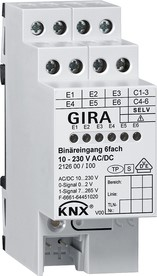
\includegraphics[width=0.2\textwidth]{figures/entradas_apertura.jpg}   
	\caption{Módulo 6 entradas para sensores de apertura}
	\label{fig:entradas_apertura}
	\end{figure}
	\end{itemize} 
\end{itemize} 

\subsection{Pasarelas}

\begin{itemize}
\item \textbf{Para sistema de aerotermia:} 
	\begin{itemize}
	\item\underline{Descripción:} pasarela Daikin – KNX.
	\item \underline{Características:} permite la comunicación bidireccional entre los sistemas Daikin VRV y las instalaciones KNX. 
	\item \underline{Funcionalidad:} su principal misión será la de servir de puente de comunicación entre el sistema propio de los sistemas de fancoil de la vivienda y el sistema domótico KNX, permitiendo así su control a través del bus mediante el envío de telegramas y su decodificación.
	\begin{figure}[H]
	\centering
	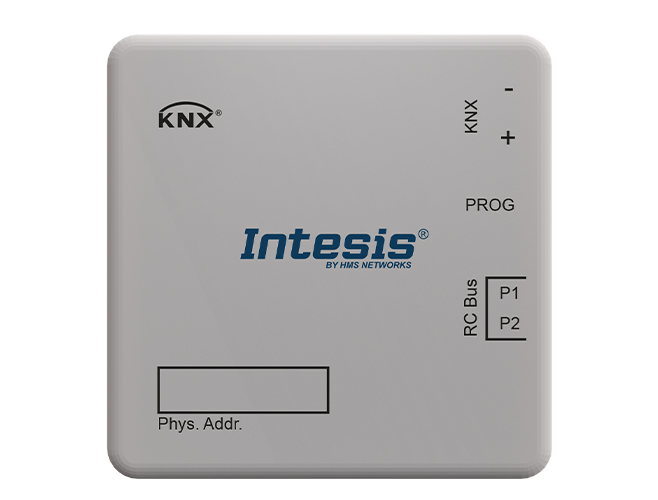
\includegraphics[width=0.47\textwidth]{figures/pasarela.png}   
	\caption{Pasarela para sistema de aerotermia}
	\label{fig:pasarela}
	\end{figure}
	\end{itemize} 
\end{itemize} 

\subsection{Servidores}

\begin{itemize}
\item \textbf{X1:} 
	\begin{itemize}
	\item\underline{Descripción:} servidor de visualización para terminales móviles.
	\item \underline{Características:}  este mecanismo permite la visualización de una interfaz personalizada en tu móvil o tablet  a través de internet, así como el control de hasta 250 funciones mediante el uso de comandos de voz o bien mediante la aplicación. Capacidad de uso de hasta 250 temporizadores, 36 bloques lógicos diferentes y 1450 datapoints.
	\item \underline{Funcionalidad:} contendrá los módulos lógicos programados para desarrollar las funcionalidades especiales del resto de módulos y el software sobre el que se programa la interfaz de visualización tanto del G1 como de la aplicación móvil. También permitirá la conexión remota a través de la aplicación móvil al alojar un servidor propio a través de la conexión Wi-Fi de la vivienda.
	\begin{figure}[H]
	\centering
	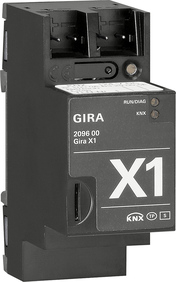
\includegraphics[width=0.23\textwidth]{figures/x1.png}   
	\caption{X1}
	\label{fig:x1}
	\end{figure}
	\end{itemize} 
\end{itemize} 

\subsection{Fuentes de alimentación}

Esta función será desarrollada por un módulo único compartido por ambos cuadros domóticos de la vivienda. Su cometido es el de transformar la corriente alterna proveniente de la acometida pública que llega a las casas con una tensión de 230V entre fase y neutro, en corriente continua de 29V, que es el potencial de bus necesario para alimentar los dispositivos. Este dispositivo no cuenta con ningún tipo de distribuidor de intensidad, por lo que la corriente nominal será repartida de manera discrecional en las salidas, hasta un máximo de 640 mA. Para prevenir posibles comportamientos anómalos de la red eléctrica, este dispositivo cuenta con una bobina de choque integrada en su interior, un componente electrónico de muy alta reactancia que hará las veces de filtro de las corrientes alternas, eludiendo futuras fallas o roturas de los mecanismos domóticos..
\begin{figure}[H]
\centering
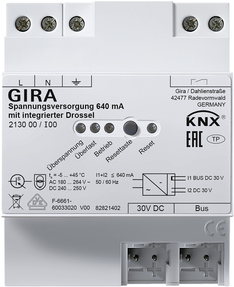
\includegraphics[width=0.3\textwidth]{figures/fuente_alimentacion.png}   
\caption{Fuente de alimentación}
\label{fig:fuente_alimentacion}
\end{figure}



\section{Dimensionamiento del proyecto}

A la hora de diseñar una instalación domótica para una vivienda, es importante no pasar por alto una serie de factores restrictivos para que todo el sistema funcione correctamente. Dos de estos parámetros que han de ser tomados en cuenta son el tamaño físico de los módulos y la demanda de potencia que reclaman.\\
 El factor limitante de tamaño viene ligado simplemente a la capacidad de alojar distintos mecanismos que permite el cuadro eléctrico de domótica. En el caso de esta vivienda, además, se ha de tener en cuenta la modularidad del sistema, por lo que la opción escogida pasa por duplicar estos armarios, conteniendo cada uno de ellos en su interior los elementos que permitiesen a los subsistemas funcionar de manera independiente en caso de querer dividir la vivienda en dos casas diferentes. El único mecanismo que compartirán ambas viviendas será la fuente de alimentación de 640 mA, por lo que la suma de demanda de corriente total no deberá nunca superar este valor. Para realizar este estudio, se han escogido las corrientes máximas que pueden llegar a demandar los mecanismos, en lugar de sus corrientes nominales, cerciorándonos así de que bajo ninguna circunstancia o condición adversa, el sistema quedará sin alimentación por una demanda de intensidad superior a la proporcionada. Para simplificar la visualización de los límites que plantean ambos parámetros, se ha elaborado una lista para facilitar esta tarea:

\begin{flushleft}
\begin{longtable}[H]{|p{4cm}|c|c|c|c|c|}
\hline 
\rule[0mm]{0mm}{5mm}
\multirow{2}{*}{Descripción}  &  \multirow{2}{*}{Cantidad} & Consumo & Tamaño & Consumo & Tamaño\\
&  &  ud. (mA) &  ud. (DIN) &  Total  (mA) & Total (DIN)\\ \hline \hline
\endhead
\rule[0mm]{0mm}{4mm}
Detect. Movimiento &  \multirow{2}{*}{4} &  \multirow{2}{*}{10} &  \multirow{2}{*}{0} &  \multirow{2}{*}{40} &  \multirow{2}{*}{0}\\
Komfort 2,2m KNX& & & & &\\
\hline
\rule[0mm]{0mm}{4mm}
Detect. Presencia  & \multirow{2}{*}{1} & \multirow{2}{*}{10} & \multirow{2}{*}{0} & \multirow{2}{*}{10} & \multirow{2}{*}{0}\\
 KNX Mini Komfort & & & & &\\
\hline
\rule[0mm]{0mm}{4mm}
Detect. Movimiento &  \multirow{2}{*}{1} &  \multirow{2}{*}{10} &  \multirow{2}{*}{0} &  \multirow{2}{*}{10} &  \multirow{2}{*}{0}\\
 KNX Standard 2,2m & & & & &\\
\hline
\rule[0mm]{0mm}{4mm}
\rule[0mm]{0mm}{4mm}
Sensor CO2 +  & \multirow{2}{*}{1} & \multirow{2}{*}{25} & \multirow{2}{*}{0} & \multirow{2}{*}{25} & \multirow{2}{*}{0}\\
Humedad KNX & & & & &\\
\hline
\rule[0mm]{0mm}{4mm}
Pulsador KNX de 2 elem. &  \multirow{2}{*}{37} &  \multirow{2}{*}{5} &  \multirow{2}{*}{0} &  \multirow{2}{*}{185} &  \multirow{2}{*}{0}\\
con mando de 1 punto  & & & & &\\
\hline
\rule[0mm]{0mm}{4mm}
Fuente alimentacion & \multirow{2}{*}{1} & \multirow{2}{*}{-640} & \multirow{2}{*}{4} &  \multirow{2}{*}{(-640*)} & \multirow{2}{*}{4}\\
 640mA KNX  & & & & &\\
\hline
\rule[0mm]{0mm}{4mm}
Actuador de conmutación   &  \multirow{2}{*}{2} &  \multirow{2}{*}{24} &  \multirow{2}{*}{12} &  \multirow{2}{*}{24} &  \multirow{2}{*}{12}\\
24 outs / 12 persianas 16A  & & & & &\\
\hline
\rule[0mm]{0mm}{4mm}
Actuador calefaccion & \multirow{2}{*}{2} & \multirow{2}{*}{12} & \multirow{2}{*}{4} & \multirow{2}{*}{48} & \multirow{2}{*}{8}\\
6 elementos KNX & & & & &\\
\hline
\rule[0mm]{0mm}{4mm}
Entrada binaria KNX de &  \multirow{2}{*}{4} &  \multirow{2}{*}{7,5} &  \multirow{2}{*}{2} &  \multirow{2}{*}{30} &  \multirow{2}{*}{8}\\
 6 elem. 10-230 V CA/CC & & & & &\\
\hline
\rule[0mm]{0mm}{4mm}
 Detector de humos & 4 & 0  & 0 & 0 & 0\\
\hline
\rule[0mm]{0mm}{4mm}
Gira X1 & 1 & 10 & 2 & 10 & 2\\
\hline
\rule[0mm]{0mm}{4mm}
Gira G1 & 1 & 0 & 0 & 0 & 0\\
\hline
\rule[0mm]{0mm}{4mm}
Actuador de regulacion  &  \multirow{2}{*}{4} &  \multirow{2}{*}{15} &  \multirow{2}{*}{4} &  \multirow{2}{*}{60} &  \multirow{2}{*}{16}\\
4 elementos Komfort KNX & & & & &\\
\hline
\rule[0mm]{0mm}{4mm}
Interfaz KNX para &  \multirow{2}{*}{2} &  \multirow{2}{*}{15} &  \multirow{2}{*}{2} & \multirow{2}{*}{30} & \multirow{2}{*}{4}\\
contadores de consumo  & & & & &\\
\hline
\rule[0mm]{0mm}{4mm}
Panel táctil capacitivo con display & 6 & 25 & 0 & 150 & 0\\
\hline
\rule[0mm]{0mm}{4mm}
Actuador de clima con &\multirow{2}{*}{2} & \multirow{2}{*}{10} & \multirow{2}{*}{4,5} & \multirow{2}{*}{20} & \multirow{2}{*}{9}\\
zonificación de 4 zonas   & & & & &\\
\hline
\rule[0mm]{0mm}{4mm}
Medidor de energía  & \multirow{2}{*}{2} & \multirow{2}{*}{17,5} & \multirow{2}{*}{2} & \multirow{2}{*}{35} & \multirow{2}{*}{4} \\
eléctrica KNX KES Plus & & & & &\\
\hline
\hline
\rule[0mm]{0mm}{4mm}
 & & &\textbf{TOTALES}&691 (51*)&75\\
\hline
\caption{Dimensionamiento}
\label{tab:tabla_dimensionamiento}
\end{longtable}
\end{flushleft}

En la tabla anterior (\ref{tab:tabla_dimensionamiento}) aparecen elementos con un tamaño DIN igual a cero, lo que es debido, no a su inexistencia, si no a que son elementos que no se instalarán en el cuadro domótico, sino en otros lugares de la vivienda, como paredes o cajas de aplique, y por lo tanto, su tamaño no afectará al dimensionamiento final de los cuadros eléctricos, teniendo una menor repercusión a la hora de su implementación al sistema, ya que además, cuentan con un tamaño bastante reducido.\\
Otro dato relevante se presenta en el consumo total, donde aparecen dos valores: el de consumo total y entre paréntesis el balance del consumo total, en el que se ha tenido en cuenta la insuflación de intensidad de la fuente, permitiendo así conocer el margen existente en la instalación de cara a la posible implementación futura de nuevos módulos.

\section{Secciones y funcionalidad}

\subsection{Iluminación}En esta sección se agrupan todos los elementos de la vivienda que comparten el mismo desempeño: iluminar, independientemente de si se tratan de luminarias del tipo ON/OFF o del tipo regulable. Cada punto de luz se controlará de manera independiente del resto de puntos, y se podrá hacer desde uno o más de los pulsadores instalados, desde la pantalla del G1 o desde la aplicación del móvil. Se han habilitado mediante programación los llamados servicios centralizados, permitiendo así controlar conjuntos de luminarias como por ejemplo, el centralizado general, que permite apagar todas las luces de la vivienda, permitiendo así al cliente poder salir de la vivienda con la seguridad de no estar malgastando energía, ahorrando de esta manera en su factura eléctrica. \\\\ Para esta sección también se ha hecho uso de los sistemas sensoriales de movimiento, presencia y luminosidad: la luminaria del trastero, las de los pasillos y el hall se encienden de manera automática al detectar movimiento en ellos; en el salón, sin embargo, se ha utilizado un detector de presencia al no tratarse de una zona de paso, sino de permanecer en ella sin reealizar grandes movimientos, que en combinación con la cuantificación de luminosidad en la estancia, enciende de manera automática la lámpara si detecta a alguna persona y regula su intensidad luminica en función del valor de luminosidad sensado.\\
\subsection{Recuperador de CO\textsubscript{2}}Esta sección contará con un detector de partículas de CO\textsubscript{2} que activará la señal para dar la orden a un sistema de extracción y renovación de aire mediante un sistema de ventiladores. De manera habitual, el sistema de recuperación debe permanecer en funcionamiento con el menor nivel de ventilación activado, y deberá ser apagado y reactivado por el cliente de manera manual mediante un switch habilitado tanto en la G1 como en la aplicación del móvil. \\ 
Si el sistema se encuentra operativo, el sensor lanzará señales de activación de los diferentes niveles de velocidad de los ventiladores en función de la cantidad de partículas detectadas. Concretamente, se han programado tres límites: el primero de ellos, cuando se detectan entre 500 y 1000 partículas de CO\textsubscript{2} por millón analizadas, un segundo limite que activa el siguiente nivel de velocidad de los ventiladores cuando detecta entre 1000 y 1500 partículas por millón, y finalmente el tercer limite, que activa la máxima velocidad al detectar una cantidad superior a las 1500 partículas por millón. Por añadidura, al activar cualquier luz de alguno de los baños, el ventilador entrará en velocidad máxima durante 10 minutos, independientemente de los valores sensados, al igual que al accionar una de las teclas de los pulsadores, que ha sido programada para lanzar esta función de recuperación.\\
\subsection{Ventanas, persianas y proyector}Desde esta sección se efectuara un control sobre los motores embebidos en las cajas de las persianas y en las ventanas. La programación desarrollada permitirá al usuario el cierre o la apertura total del elemento a controlar, así como su posicionamiento en un lugar concreto de su recorrido en función de un porcentaje de su tiempo total de apertura.\\
\subsection{Seguridad ante incendios: }esta sección contará con detectores de humo instalados en diferentes habitaciones de la vivienda, que una vez activados, enviarán una señal de activación a la sirena de alarma y cortarán el suministro de gas mediante el cierre de la electroválvula. Esta alarma enviará una notificación tipo Push a los dispositivos móviles conectados con la instalación, permitiendo la desactivación de la señal acústica, manteniendo el cierre de la electroválvula.\\
\subsection{Seguridad ante intrusiones: }para evitar en la medida de lo posible la irrupción de personas no deseadas en la vivienda, esta sección hace uso de los sensores de movimiento y presencia utilizados en la sección de iluminación, para lanzar la señal de alarma que activa la sirena y envía un mensaje Push a los dispositivos móviles conectados con la aplicación cuando se active el modo \textit{"Fuera de casa"} o \textit{"Vacaciones"}.\\
\subsection{Seguridad ante inundaciones}Esta sección tendrá un funcionamiento similar a la referida a seguridad frente incendios, únicamente cambiarán los sensores de humo por otros de inundación, que estarán ubicados en las zonas húmedas de la casa, como son los baños y la cocina.\\
\subsection{Clima} \label{sec:sec_clima} Esta sección será la encargada de controlar la temperatura de la vivienda haciendo uso de diversos elementos. Entre ellos encontramos los termostatos, que harán las veces de interfaz con el usuario en cada habitación gracias a sus pulsadores y displays, permitiendo controlar la velocidad de los ventiladores en caso de que se encuentren en funcionamiento, controlar si se desea o no aclimatar esa estancia y que temperatura es la requerida por el cliente. Internamente, también se encargará de gestionar al resto de equipos, indicando cuando y como deben encenderse, y actuar en función de la temperatura sensada y la temperatura de consigna deseada. \\
Durante el verano, el equipo de refrigeración se basará únicamente en el uso del equipo de fancoil, evitando así la aparición de hongos y humedades producidos por la condensación proveniente del uso del suelo radiante con agua fría. El usuario podrá elegir entre dos modalidades de actuación: la manual, en la que podrá seleccionar entre tres niveles la velocidad a la que desea que se expulse el aire refrigerado por el equipo fancoil, o bien el modo automático, en el que el módulo de actuación de las rejillas seleccionará de entre las tres velocidades mencionadas anteriormente una de ellas en función de un factor de ponderación. Este factor, limitado a un máximo de 100 puntos, será implementado durante su programación, dotando de un valor numérico a cada habitación en función de diversos parámetros como pudiera ser su tamaño o el nivel de confort que requiera. Un ejemplo claro de esto pudiera ser la actuación de uno de los equipos instalados que se encargaría de controlar la temperatura de la cocina, el salón y una de las habitaciones, a los que se les ha otorgado una ponderación de 15 puntos, 55 puntos y 30 puntos respectivamente. Si en una primera situación, hubiese demanda de la cocina y la habitación, al sumar 45 puntos no llegarían al requerimiento del segundo nivel de velocidad, activando así únicamente el primer nivel; mientras que si se activasen cocina y salón simultáneamente, al superar el baremo, sí que entraría en funcionamiento la segunda velocidad del equipo.
\bigskip
\begin{table}[H]
\begin{center}
\begin{tabular}{| c | c |} \hline
\rule[0mm]{0mm}{6mm}
\textbf{Valor ponderado de demanda} & \textbf{Nivel activo} \\ \hline
\rule[0mm]{0mm}{4mm}
0 & OFF \\ \hline
\rule[0mm]{0mm}{4mm}
1-33 & Velocidad 1 \\ \hline
\rule[0mm]{0mm}{4mm}
34-66 & Velocidad 2 \\ \hline
\rule[0mm]{0mm}{4mm}
67-100 & Velocidad 3 \\ \hline
\end{tabular}
\caption{Ponderación velocidad fancoils}
\label{tab:vel_fancoils}
\end{center}
\end{table}
En cambio, durante el modo invierno el equipo principal que actuará será el de suelo radiante. En este caso el termostato se encargará de enviar una orden de apertura a las válvulas de las habitaciones en las que la temperatura se encuentra por debajo de la demanda, y una señal de arranque a la caldera en cuanto que una de estas válvulas es abierta, haciendo circular el agua caliente a través del entramado de tuberías instaladas en el suelo. En el momento que la temperatura de la habitación y la de consigna tienen una diferencia mayor de 3ºC, se ha programado el comienzo de actuación del sistema secundario: el sistema de fancoil. El sistema de aerotermia tendrá exactamente el mismo modo de funcionamiento que en el modo verano, activando sus velocidades en función de la ponderación de las habitaciones que se encuentren en demanda al encontrarse funcionando en modo automático, o pudiendo ser elegida por el usuario en el modo manual. \\\\
Para evitar el uso prolongado e indebido de los equipos que componen el sistema, se han programado un control del tipo proporcional integral (PI), debido a que se ajusta mejor al comportamiento que este ofrece frente a la alternativa del control de dos puntos con histéresis. Se trata de un método de control regido por un algoritmo de control lineal basado tanto en la diferencia entre las temperaturas de consigna y de referencia como en los datos del histórico del sistema, reduciendo así las franjas de oscilación de la temperatura del habitáculo, estabilizando paulatinamente su valor en el entorno de la temperatura de consigna establecida por el usuario. \\\\
Como se puede apreciar en la Imagen \ref{fig:metodos_control}, se ofrece una comparativa entre los dos métodos de control para que el sistema proporciona a la estancia una temperatura de 25ºC. Por el método, descartado, de control mediante dos puntos se establecen los límites inferior y superior de temperatura en los que el sistema debe encenderse y apagarse, respectivamente. Con este método más sencillo de programar, el sistema no se encuentra funcionando constantemente, pero sufre picos de alto consumo energético para alcanzar el límite superior desde una temperatura ligeramente menor al límite inferior, con el añadido de que la estancia se encuentra, casi en la totalidad del tiempo, lejos de la temperatura de consigna. En cambio, el método de control proporcional integral, se encuentra constantemente en funcionamiento, y trabaja regulando la temperatura de exhalación del aire para mantener la temperatura en un valor más ajustado al de consigna de manera constante, sin provocar tiempos de funcionamiento a marchas forzadas de la máquina de aerotermia o de la caldera, evitando así los picos de alta demanda energética por parte del sistema. 
\bigskip
\begin{figure}[H]
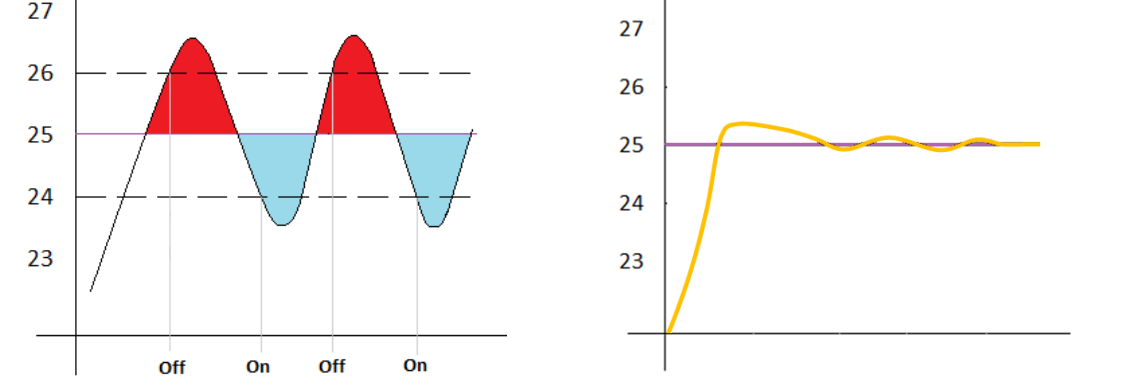
\includegraphics[width=1.15\textwidth]{figures/metodos_control.png}   
\caption{Comparación entre control de dos puntos con histeresis [izq] y control PI [dcha]}
\label{fig:metodos_control}
\end{figure}
\bigskip
La programación de este algoritmo requerirá de la configuración de tres parámetros esencialmente:
	
	\begin{itemize} 
	\item La constante de proporcionalidad (K) expresada en grados centígrados, encargada de que el error estacionario se 	reduzca a cero produciendo el menor valor posible de sobreoscilación de la señal. 
	\item El tiempo integral (T) expresado en minutos, será un valor asociado a la inercia térmica del sistema de aerotermia que 				permite ajustar el error de aproximación en función del tiempo transcurrido, es decir, la velocidad de impacto que tiene el 	sistema para variar la temperatura.
	\item El tiempo de ciclo, también expresado en minutos, que condicionará la frecuencia de muestro y actualización de la señal de 			control enviada tanto a la caldera como a las máquinas de aerotermia.
	\end{itemize} 
Se ha establecido un valor de K=4 y T=90min. tanto para el modo enfriar como calentar de la máquina de aerotermia, mientras que para el suelo radiante, los valores escogidos han sido K=5 y T=240min. El tiempo de ciclo que se ha encontrado más optimizado respecto a las condiciones de ahorro energético y confort térmico ha sido de 15min. \\
El control de los sistemas de fancoil normalmente se ejecuta a través de comunicaciones vía infrarrojos, protocolo que no entra dentro del alcance de la tecnología KNX, por lo que ha sido necesaria la implementación de un sistema de pasarelas para poder establecer el nexo de comunicación entre el equipo y el bus KNX de manera remota, sin uso de señales infrarrojas. Esta pasarela será conectada al mando de control original de la máquina de aerotermia, que no será removido de la instalación debido a su alta fiabilidad a la hora de identificar los posibles errores o fallos que sufra el equipo. Adicionalmente, el cliente tendrá la opción de cambiar entre modo invierno/verano desde la pantalla del G1 o desde la aplicación del móvil, en función de si desea que el sistema proporcione calor o frio, respectivamente.\\
\subsection{Consumos} Por petición del cliente, se debe hacer un seguimiento de los consumos tanto de luz, como de agua y gas que se dan en la vivienda, por lo que se han habilitado lectores adicionales a los respectivos instalados por las compañías de suministro, permitiendo visualizar en la pantalla del G1 o en la aplicación del móvil el consumo instantáneo de tensión, corriente, potencia, agua o gas; el consumo total de energía, de agua y gas durante diversos periplos, como por ejemplo el consumo del mes anterior, el consumo desde el día 1 del mes en el que se encuentren o incluso en un periodo definido por el propio usuario.

\section{Ubicación}

Otro de los factores clave para poder hacer un diseño funcional y con el menor número posible de fallos, es la ubicación física de los módulos que no van acoplados en el cuadro eléctrico de la domótica, aquellos que se encuentran repartidos por distintos puntos de la vivienda, como en los techos, paredes (tanto en su interior como en su cara exterior) o incluso en el exterior de la vivienda. Este factor toma especial relevancia por el tiempo necesario para la recepción de los telegramas por parte de los módulos más alejados, y la posibilidad de que estos se solapen y generen acuses de recibo no veraces, provocando discrepancias entre el valor que el sistema cree que posee esa variable y el valor del estado en que se encuentra realmente. Otro factor afectado por la ubicación lejana, es la transmisión de los valores medidos por los sensores, ya que si el módulo de entradas se encuentra alejado de él, pueden producirse cambios en la tensión transmitida, dando lugar a una lectura incorrecta de las magnitudes sensadas.
\begin{figure}[H]
\begin{center}
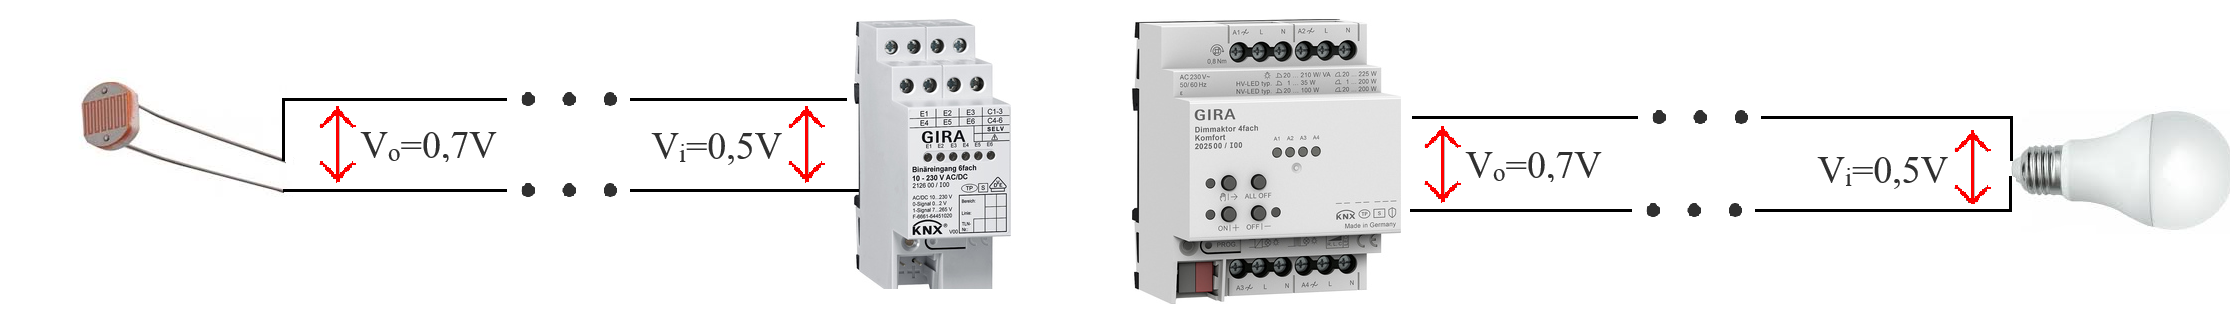
\includegraphics[width=1.15\textwidth]{figures/caida_tension.png}   
\caption{Error de tensión debido a la distancia}
\label{fig:caida_tension}
\end{center}
\end{figure}
Para evitar este tipo de errores, se realiza una planificación de la ubicación de los elementos para que ninguno de ellos se encuentre demasiado lejos de su receptor, dando lugar a los siguientes planos:\\\\\\
La ubicación respecto del resto de elementos de la vivienda también es un factor a tener presente a la hora de realizar el diseño previo de la instalación, ya que de no tenerse en cuenta podría dar lugar a funcionamientos inesperados, la inhabilitación del mecanismo o llegar incluso a provocar situaciones de peligro para el usuario. El caso del detector de humos es uno de ellos, y es que una colocación incorrecta podría dar lugar a que el sensor no detectarse los cambios en la temperatura de la habitación o que al contar esta con grandes dimensiones, no fuese capaz de detectar la presencia de humos nocivos para la salud adecuadamente. Es por ello que, y siguiendo las recomendaciones del fabricante, estos sensores deberán colocarse en el centro de una habitación no más grande de 60 m\textsuperscript{2} y a una distancia mínima de 50 centímetros  otros elementos como lámparas o paredes, sin superar los 6 metros de altura. \\\\
Los detectores de inundación también deberán ser instalados siguiendo una serie de pautas para asegurar su correcto funcionamiento. Entre otras normas, se puede destacar que debe colocarse de manera sobre una superficie que no tenga una inclinación demasiado pronunciada, siendo óptimo que esta sea totalmente horizontal y al nivel más bajo posible de altura tal y como se muestra en la imagen \ref{fig:local_inundacion}, debido a que será necesario el contacto físico entre el sensor y el elemento líquido para hacer saltar la alarma. Es importante también una situación de cercanía con las fuentes de caudal y los electrodomésticos o elementos sobre los que se desea hacer el control, ya que la detección de la fuga será más temprana. Pese a su reducido tamaño, se deberá contar con el espacio que ocuparán estos sensores a la hora de la planificación.
\begin{figure}[H]
\begin{center}
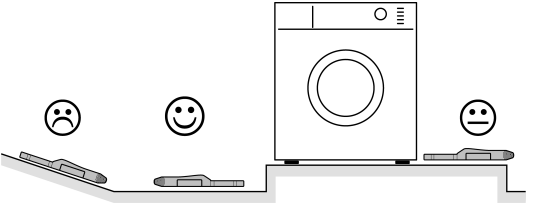
\includegraphics[width=0.85\textwidth]{figures/local_inundacion.png}   
\caption{Ejemplos de posicionamiento de los sensores de inundación}
\label{fig:local_inundacion}
\end{center}
\end{figure}
Otro ejemplo de la importancia de la ubicación de los elementos la encontramos en los sensores de movimiento de tipo PIR: la geometría de la lente que lo recubre le permite detectar la radiación térmica con un amplio margen de amplitud, unos 180º aproximadamente. Esta capacidad será aprovechada al máximo siguiendo una serie de criterios como, por ejemplo, la altura a la que se encuentre y la posición en la habitación respecto de otros enseres que en ella se encuentren. Según las indicaciones del fabricante, el sensor debe ser colocado a una altura de 2,20 m con una leve inclinación hacia el suelo, permitiendo así una mayor dispersión de los haces detectores por la sala. También es necesario tener en consideración el tipo de movimiento que se va a realizar en las salas donde van a ser instalados, ya que el alcance de estos sensores varía en función de si se trata de un movimiento de tipo radial o tangencial.
\begin{figure}[H]
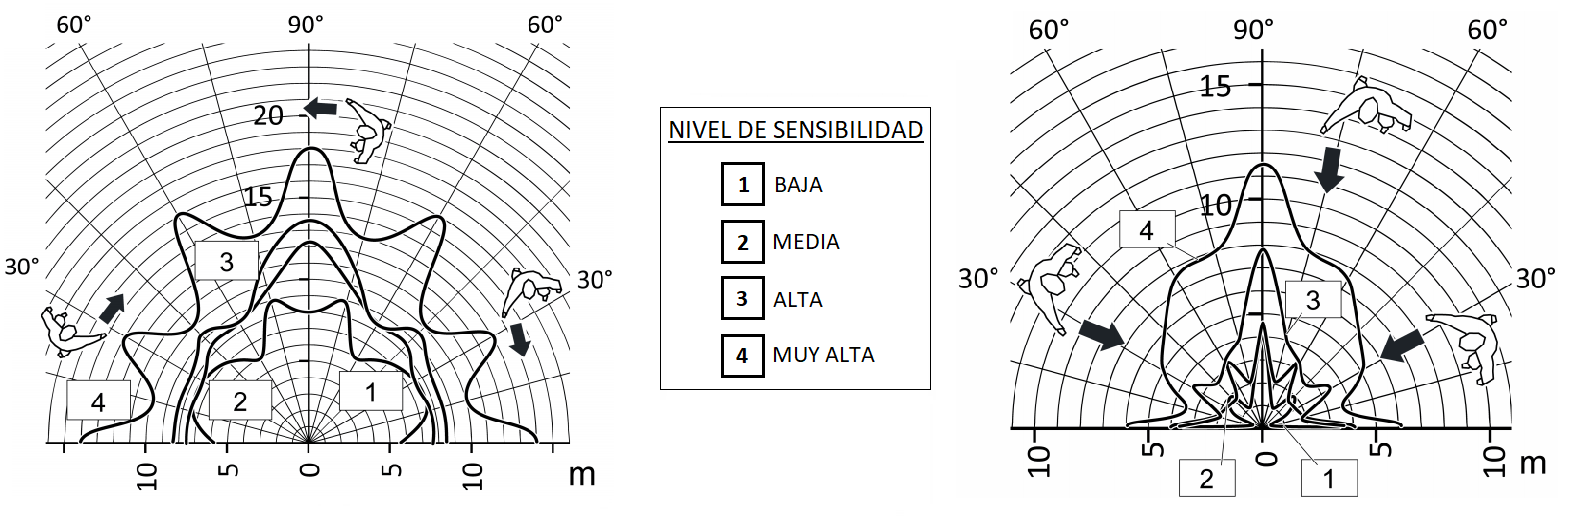
\includegraphics[width=1.15\textwidth]{figures/alcance_PIR.png}   
\caption{Alcances del sensor PIR para movimiento tangencial [izq] y radial [dcha]}
\label{fig:alcance_PIR}
\end{figure}

Como la función que tienen asignada estos sensores es la de detectar el movimiento en los pasillos y el hall de la vivienda para activar la orden de encendido de las luces, se han colocado estratégicamente en los extremos de los pasillos, aprovechando su alta sensibilidad ante el movimiento radial, que es el más usual en este tipo de espacios. En cuanto a los sensores que se encuentran en el hall y el trastero, se han situado en lo alto de las paredes situadas enfrente de las puertas de acceso, para encender las luminarias en el momento que estas son abiertas.\\
En el caso de detector de presencia instalado en el salón se cuenta con un radio de detección de 360º, por lo que será instalado en el centro del techo de la sala. Al tratarse de una vivienda antigua, el techo se cuenta con una altura considerable (aprox 3,50m), lo que supondrá una ventaja, ya que de igual manera que los sensores de movimiento, al colocarse en una posición más elevada, se obtiene una mayor distancia de detección, siempre teniendo en cuenta el tipo de movimiento que se desee detectar:
\begin{figure}[H]
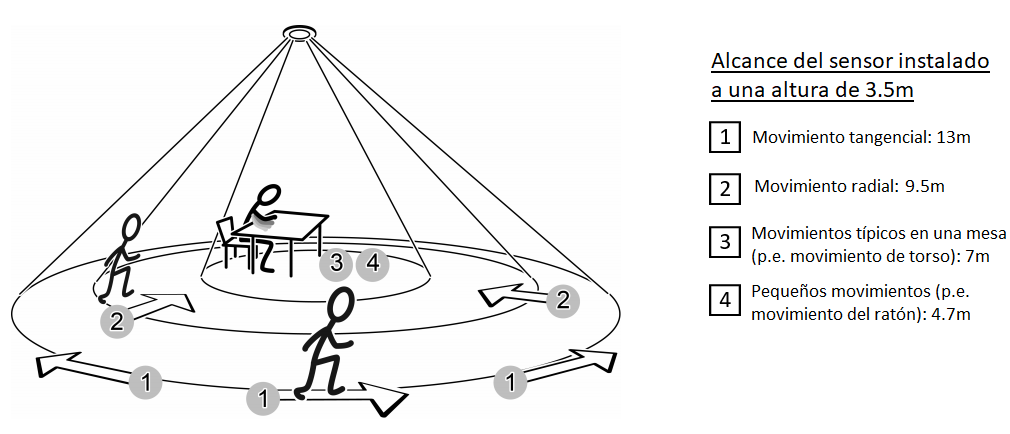
\includegraphics[width=1.15\textwidth]{figures/alcance_presencia.png}   
\caption{Alcances del sensor de presencia}
\label{fig:alcance_presencia}
\end{figure}

\section{Conexionado}
En esta sección del documento se detallará el conexionado del cuadro de domótica, incluyendo el cableado desde la toma de corriente de línea desde el cuadro eléctrico hasta los propios elementos. A causa de a las grandes dimensiones que poseería el esquema eléctrico real debido a la multitud de mecanismos conectados, se ha decidido hacer un esquema simplificado que muestre como se realizan las conexiones a cada uno de los elementos, pudiendo ser replicada la instalación real completa utilizando las tablas de conexionado de elementos del Anexo~\ref{aped.B}. A continuación se fragmenta en diferentes puntos las conexiones existentes en la instalación para ser vistas en más detalle:
\begin{itemize}
\item \textbf{Cuadro eléctrico de domótica } \\ \\
Siguiendo las normas de seguridad recogidas en la normativa \cite{Reglamento:2021}, una de las líneas del sistema trifásico y el neutro de la instalación eléctrica del edificio se hacen pasar en primera instancia por un Interruptor General Automático (IGA), ya que el Interruptor de Control de Potencia (ICP), encargado de cortar el suministro en situaciones de sobrecarga, cortocircuito y en los que la demanda de potencia supera a la potencia contratada, se encuentra integrada en el contador instalado en la vivienda por la compañía de suministro eléctrico. El IGA tendrá como misión principal proteger el resto del circuito en el caso de que se produzca un cortocircuito o se supere la potencia máxima que es capaz de soportar la instalación, como por ejemplo, cuando son conectados demasiados electrodomésticos a la vez. Esta interrupción de la corriente nada tendrá que ver con cuestiones económicas o limitantes en función de lo que se tenga contratado y se pague a la compañía de suministro eléctrico, si no que será limitante en cuanto a las características físicas de la propia instalación, no pudiendo ser mejorada si no son sustituyendo y mejorado alguno de los elementos que la componen. A continuación, se ha instalado un Protector Contra Sobretensiones (PCS), que tal y como indica su nombre será el encargado de proteger el resto de circuitos en las ocasiones en las que se produzcan picos elevados de tensión no controlados, como puede ser el caso del impacto de un rayo, desviando la corriente hacia la toma de tierra, evitando daños en los equipos conectados, en la propia instalación o incluso sobre los usuarios que se encuentran en el interior de la vivienda.\\\\
Siguiendo el cableado, el siguiente elemento que nos encontramos es el Interruptor Diferencial (ID). Este elemento desarrollará la función de proteger a los usuarios de las fugas de corrientes a tierra que pudiesen producirse por daños o malas conexiones de los electrodomésticos con la instalación eléctrica. En cada vivienda es usual instalar entre dos y tres ID que agrupen varios sistemas con diferentes funcionalidades, facilitando así localizar que la fuga de corriente se está produciendo en alguno de los elementos que a ella se encuentra conectado, pero debido a demanda del cliente, se ha seguido el modelo habitual de instalación aplicado en los cuadros de las viviendas de Alemania, en el que existe un ID por cada una de las funcionalidades que se desarrollan en la instalación, teniendo el sistema de iluminación su propio ID, por ejemplo. \\\\
En último lugar, y antes de comenzar conectar los elementos, se colocan los últimos elementos de protección del sistema: los Pequeños Interruptores de Potencia (PIA), o como son conocidos comúnmente, Interruptores Automáticos. Estos interruptores sí que es habitual encontrarse uno por cada grupo de elementos con la misma funcionalidad, y tendrán como misión detectar el exceso de consumo en estos grupos, desconectándose de manera automática en tal caso. También son muy útiles en el caso de querer realizar alguna modificación en un sistema concreto, ya que si es preciso desconectarlo, no afectará al resto, que podrán seguir operando de manera normal.
\end{itemize} 
 \vspace{2cm}
Una vez explicado el conexionado hasta el cuadro de domótica, se entrara en detalle el cableado de este hasta los módulos y mecanismos que componen la instalación domótica que controla la vivienda. Entre ambas partes, se han utilizado dos tipos distintos de bornas para facilitar el peinado de los cables, su distribución y organización a lo largo de los tubos y debido a que la ley vigente dictamina que no es legal ni seguro la conexión directa de cables, teniendo que realizarse está a través de algún elemento de paso y sujeción: las bornas de paso y las de distribución. Para una mayor claridad, las bornas de distribución vendrán representadas en los esquemas con un color verde, y serán utilizadas, tal y como su nombre indica, para distribuir las tensiones que llegan a los PIAs. Estas bornas cuentan con cuatro puertos interconectados entre ellos, ofreciendo así el mismo valor de tensión en cada una de sus salidas y son independientes unas bornas a otras, a menos que se haga una conexión directa entre alguno de sus puertos. \\\\
Por otro lado, las bornas de paso, representadas en color amarillo, también cuentan con cuatro puertos, pero en esta ocasión no se encuentran conectados entre ellos, si no que tienen una distribución distinta, tal y como se muestra en la imagen. En estas bornas, el segundo y cuarto puerto si cuentan con una conexión interna para así ofrecer la misma caída de tensión en ambos puntos, mientras que el primero y el tercero serán independientes. Estas salidas cuentan con conexiones laterales que les permiten conectarse a la borna contigua al encontrarse enganchadas físicamente unas a otras, sin necesidad de realizar esta conexión mediante cables. Por lo tanto, una fila de bornas de paso compartirá la misma tensión con el resto en su primer y tercer puerto, que serán los asignados a la toma de tierra y al neutro común, respectivamente. Los otros dos puertos, serán independientes del resto de bornas e irán conectadas a la fase, uno de ellos a la entrada desde el actuador y el otro al elemento que se desea controlar.

\begin{itemize}
\item \textbf{Actuadores reguladores y binarios y de persianas} 
Una vez explicado el conexionado hasta el módulo, se pasa a detallar el cableado desde este hasta el elemento a controlar. Para esta sección, se ha dividido los elementos en tres bloques en función de su conexión: en el primer bloque se encuentran todos los elementos de tipo On/Off conectados al actuador de 24 salidas, al que llegará la fase a una de sus salidas desde la borna de distribución, saliendo por el otro terminal de esa misma salida hacia la borna de paso. La conexión de estos elementos será muy simple: de la borna de paso alimentada con fase saldrá uno de los cables que irán al elemento en cuestión, volviendo desde el otro terminal al puerto del neutro de la borna. Para el segundo tipo de elementos el conexionado será idéntico a los del primer tipo, pero en esta ocasión el actuador no solo permitirá abrir o cerrar el circuito, si no que permitirá regular la corriente de salida, realizando así la función de dimmer. Por ultimo tenemos los elementos tipo ventana, que necesitaran de dos de las salidas del actuador de 24 salidas, que vendrán alimentadas desde la borna de distribución, y saldrán hacia la borna de paso. En esta ocasión, de la borna de paso será necesario sacar tres cables hacia el elemento: uno de ellos llevara el neutro, mientras que los otros dos irán conectados a los terminales que determinan si el motor de la persiana o ventana debe actuar en una dirección o su contraria. Todas estas órdenes serán transmitidas a través del cable de bus KNX al actuar sobre los pulsadores, la pantalla o la aplicación móvil.
\end{itemize}

\begin{flushleft}
\begin{figure}[H]
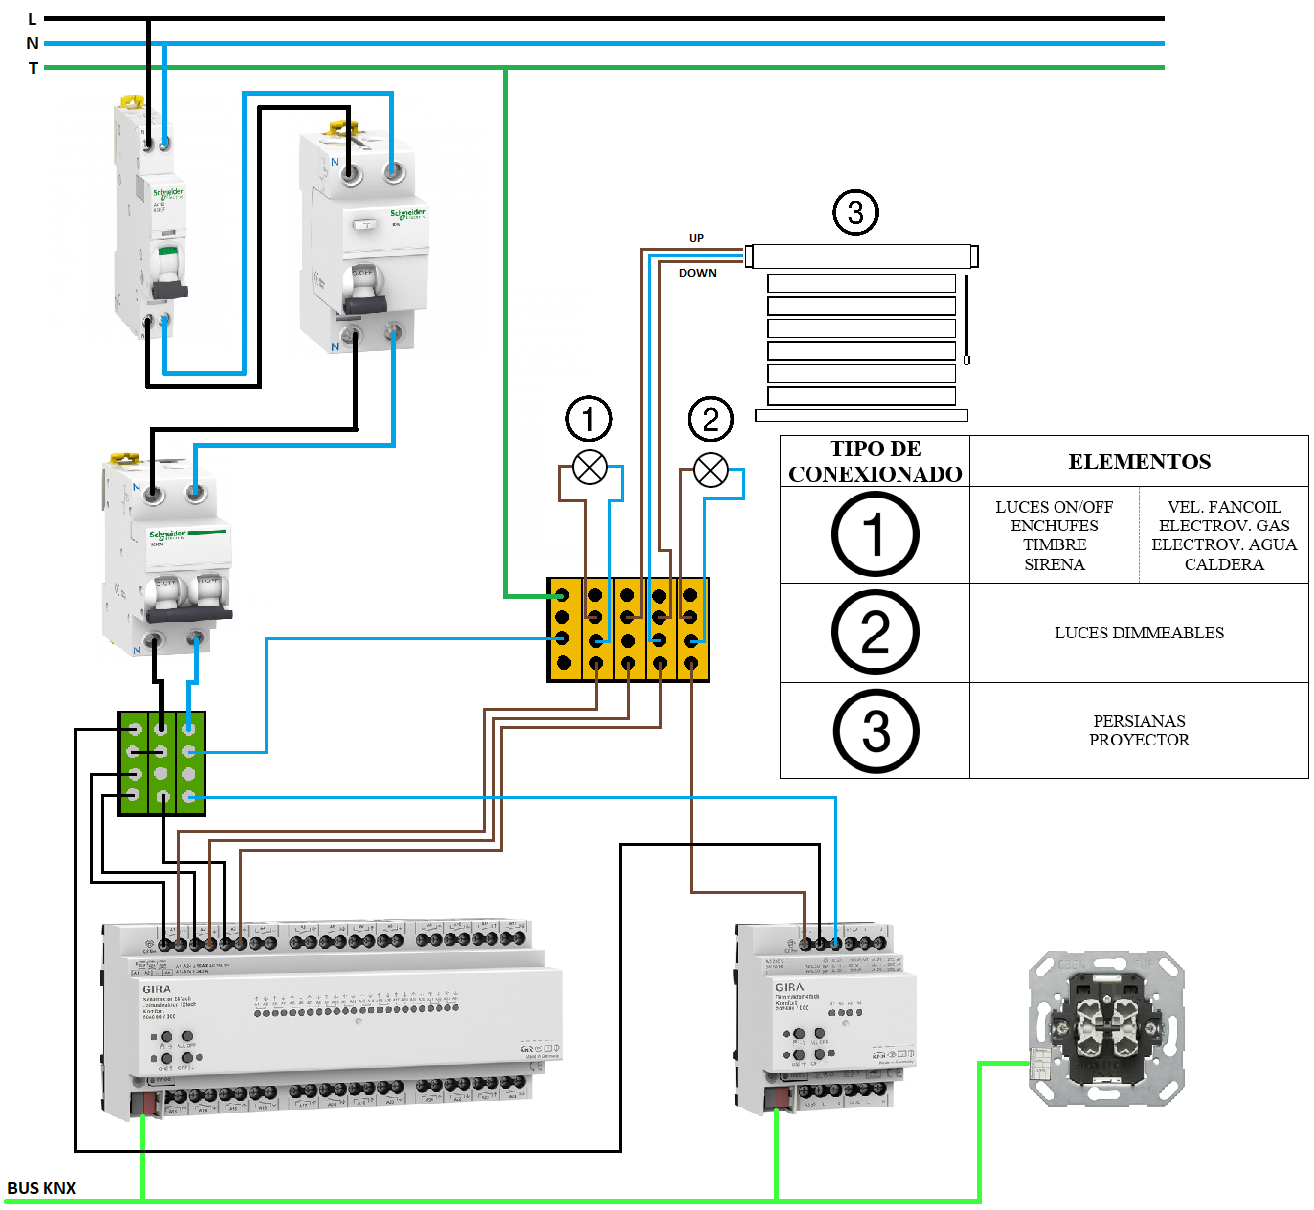
\includegraphics[width=1.15\textwidth]{figures/conex_ilu.png}   
\caption{Conexionado actuadores reguladores y binarios y de persianas}
\label{fig:conex_ilu}
\end{figure}
\end{flushleft}

\begin{itemize}
\item \textbf{Contadores de consumo} \\ \\
Para los módulos de conteo de consumo de agua y gas será necesario contar con las cajas de registro instaladas en la vivienda por la empresa suministradora, ya que este módulo no medirá los caudales de manera directa. Las cajas de registro se encuentran conectadas tanto a la caldera, para el conteo del caudal de gas, como a todas las tomas de agua de la vivienda, e irán emitiendo pulsos SO que serán cuantificados a través de un optoacoplador y transformados en un número entero a través de un factor de conversión programado en el dispositivo. \\
Por otro lado, los módulos de consumo eléctrico si realizarán el conteo de manera directa a través de los acopladores de corriente instalados en la fase de entrada de cada uno de los circuitos eléctricos que conforman la carga. Estos acopladores realizarán las mediciones mediante el uso del efecto Hall dado en los cables sobre los que se encuentran “abrazados”, por lo que será necesario planificar un espacio en los tubos de cableado que se encuentran en las paredes de la vivienda.Todas estas lecturas serán transmitidas a través del cable de bus KNX al requerir sus valores a través de la pantalla o la aplicación móvil.
\end{itemize}
\begin{flushleft}
\begin{figure}[H]
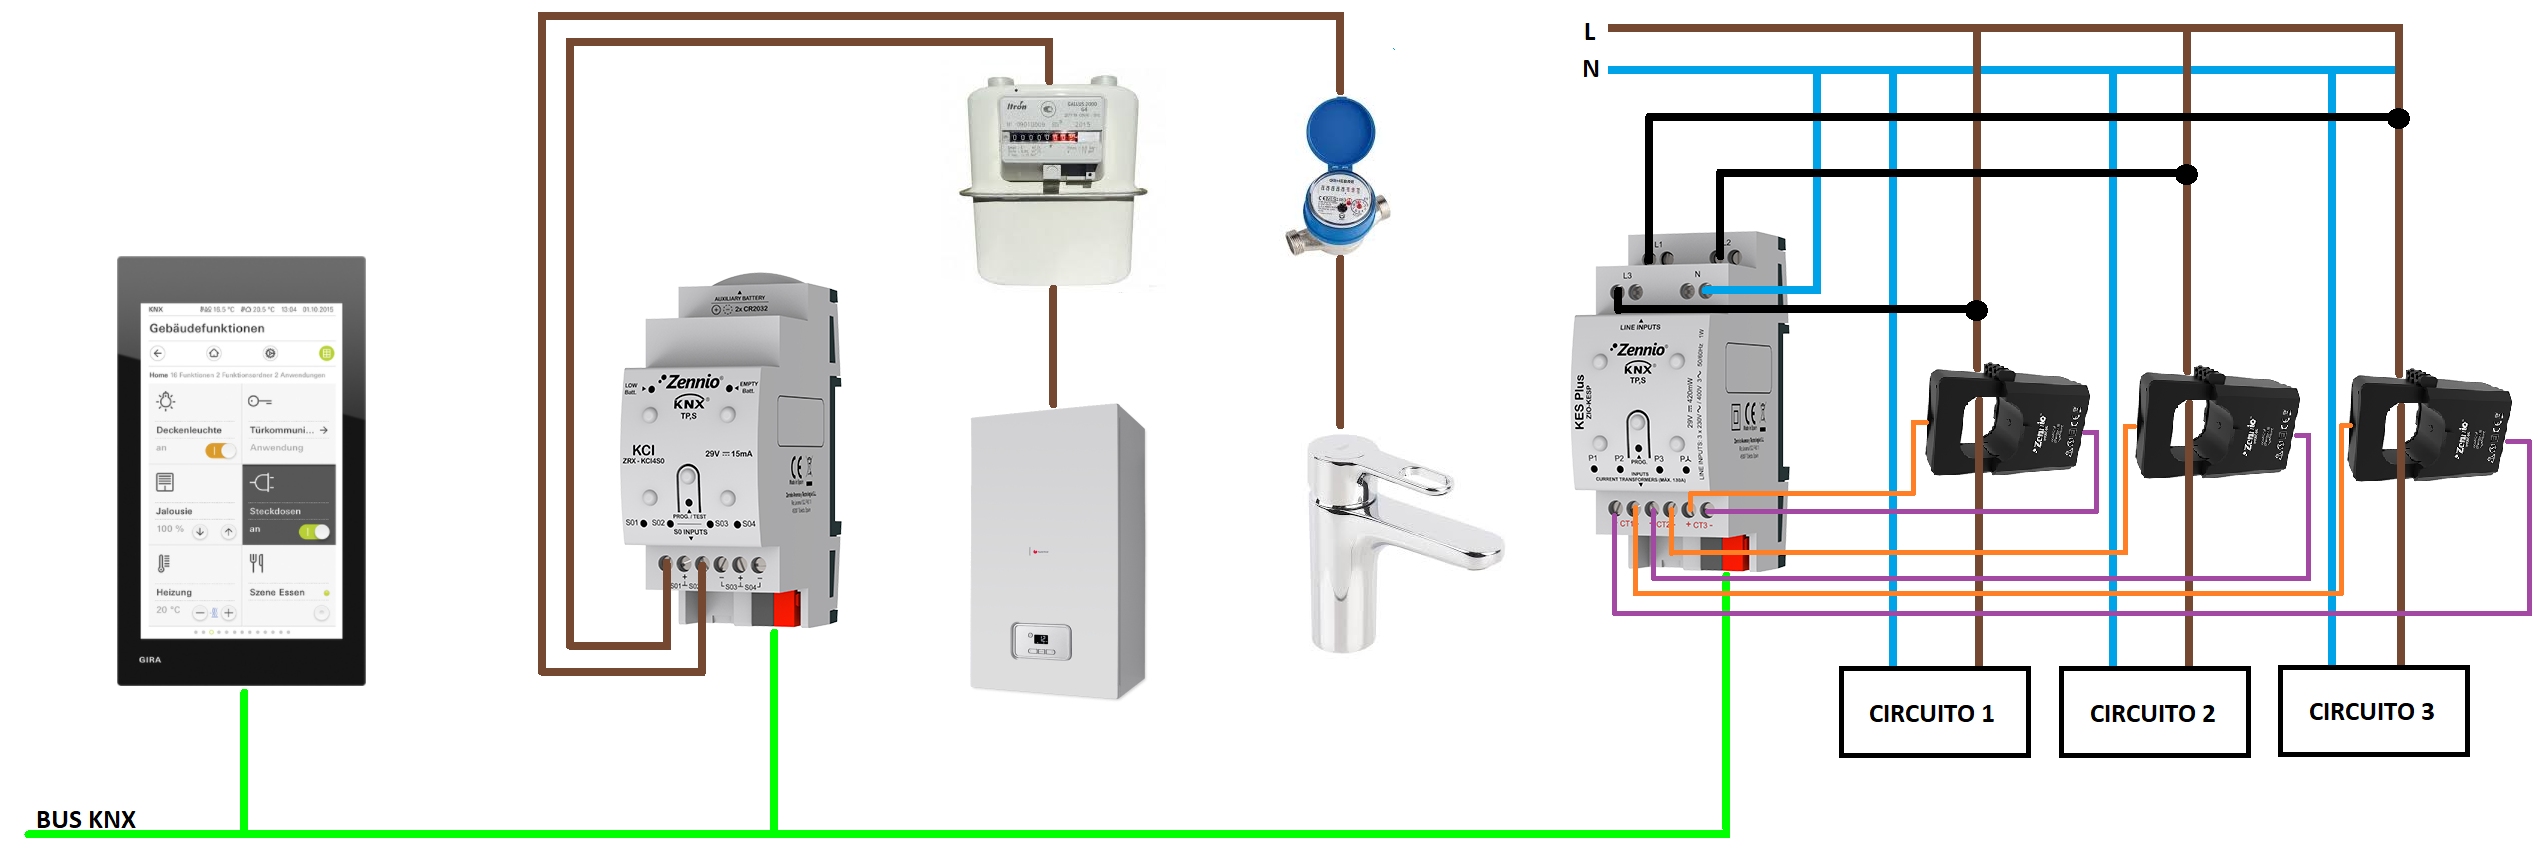
\includegraphics[width=1.15\textwidth]{figures/conex_consumo.png}   
\caption{Conexionado módulos de medidas de consumo}
\label{fig:conex_consumo}
\end{figure}
\end{flushleft}

\begin{itemize}
\item \textbf{Climatización} \\ \\
Las conexiones que se dan para los módulos encargados de la sección de climatización se dividen en bloques diferenciados por los efectores que actúan en cada uno de ellos. En primer lugar encontramos el conexionado existente para regular la apertura de las válvulas reguladoras de caudal del agua caliente que fluye a través del suelo radiante. El modulo regulador que lo controla vendrá alimentado, fase y neutro, desde las bornas de distribución conectadas al automático correspondiente. Este módulo precisa de una fuente de alimentación externa para poder controlar el porcentaje de apertura de las válvulas, por lo que su toma de alimentación también se conectará a las acometidas de fase y neutro, ya que estas válvulas necesitan alimentación de 230V para cumplir con su propósito. De cada una de sus seis salidas, saldrán el cable de tensión regulada y el de neutro hasta una borna de paso, de donde a su vez, será cableada cada una de las válvulas de regulación del suelo radiante.\\
En cuanto al módulo regulador de rejillas, este será alimentado desde una de las bornas de distribución, para así poder controlar la apertura de las mismas. Para la consecución de este objetivo, este módulo dispone de una clavija de ajuste de la tensión de salida que permite elegir entre alimentar las rejillas con 12 ó 24 voltios, siendo la primera opción la requerida para el modelo de rejillas adquirido. Esta tensión llegará a las rejillas a través de una borna de paso.\\
Por último, la pasarela para el control de la máquina de fancoil será instalada en el bus propio del sistema de aerotermia, conectada en paralelo entre el mando de control y la propia máquina. Todas estas órdenes serán transmitidas a través del cable de bus KNX al actuar sobre los termostatos, la pantalla o la aplicación móvil.
\end{itemize} 
\begin{flushleft}
\begin{figure}[H]
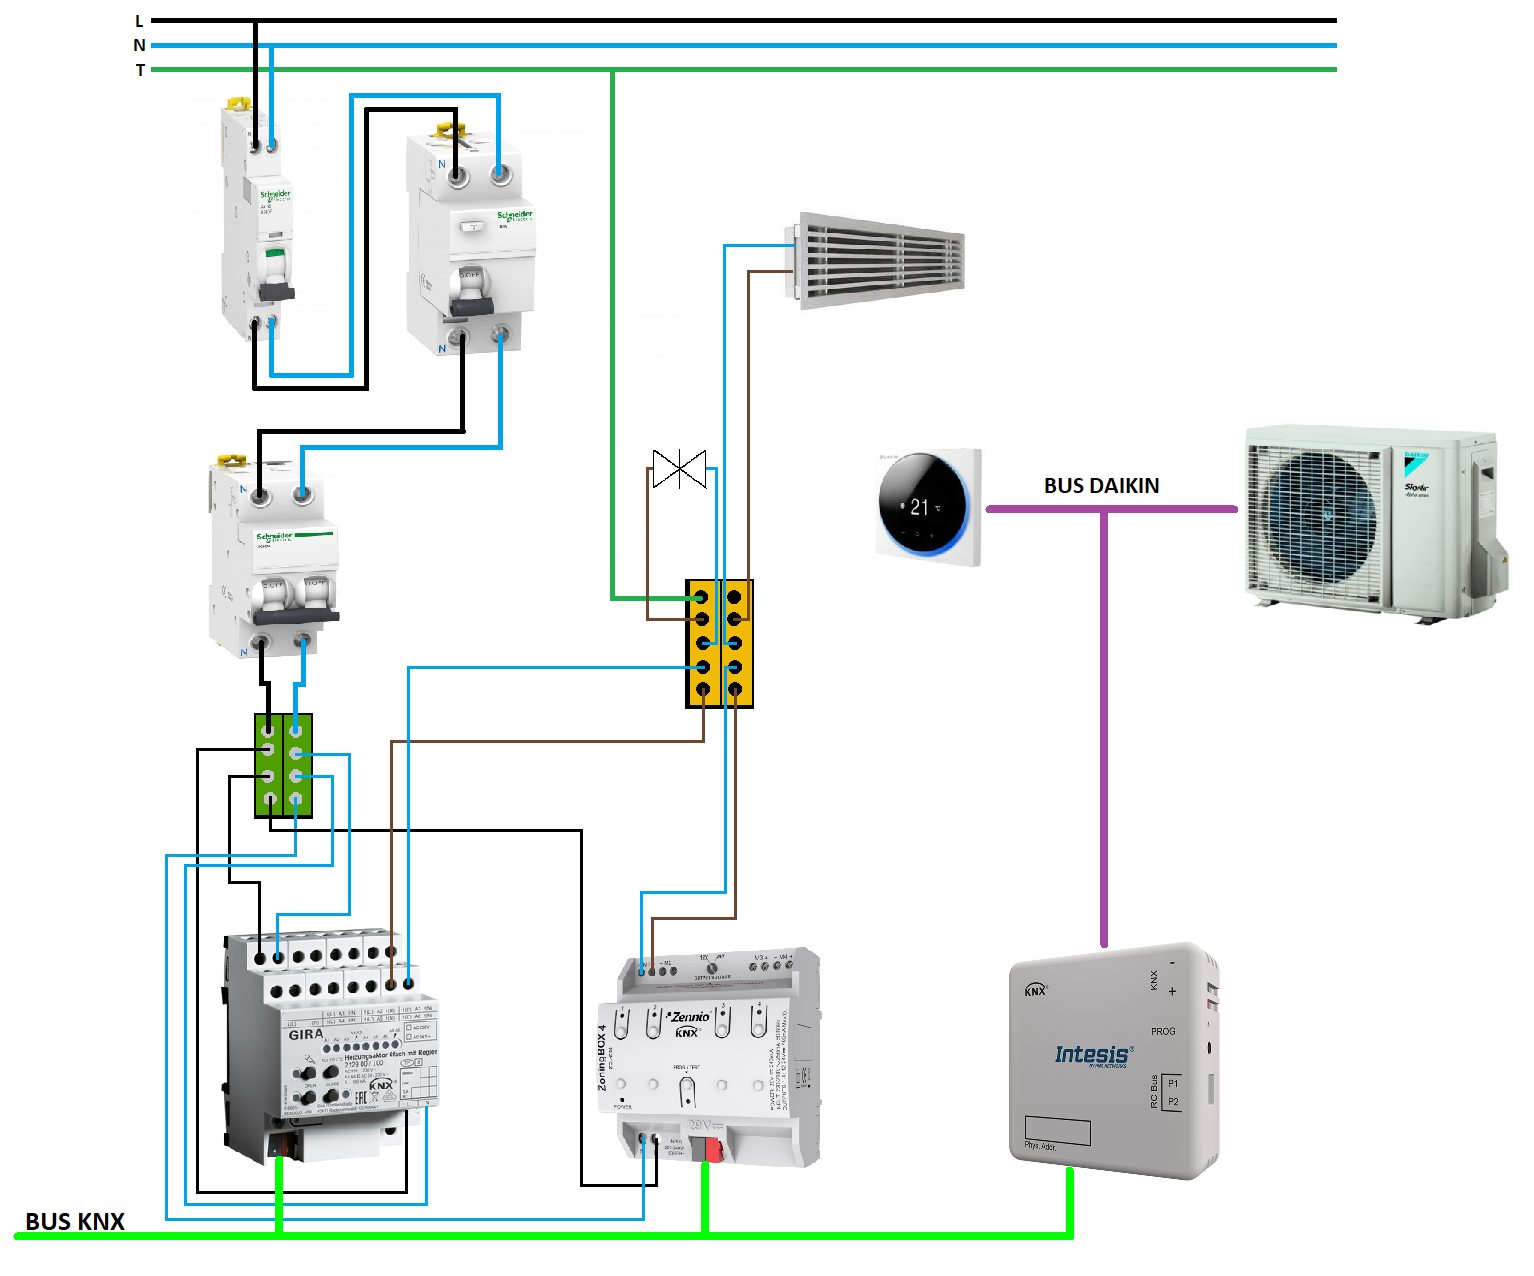
\includegraphics[width=1.15\textwidth]{figures/conex_clima.png}   
\caption{Conexionado módulos de climatización}
\label{fig:conex_clima}
\end{figure}
\end{flushleft}

\begin{itemize}
\item \textbf{Módulos sensoriales} \\ \\
Las conexiones, para el conjunto de módulos sensoriales que componen el sistema, al tratarse de módulos con la tecnología KNX integrada, serán bastante sencillas. Tanto el sensor de CO\textsubscript{2} como los sensores de movimiento y presencia irán directamente conectados al bus KNX, y desde ahí transmitirán al resto de elementos la información sensada. En cuanto al sensor de humo, lleva acoplado en su interior el módulo que le permite transmitir vía KNX tanto la alarma térmica como la de humo, por lo que tampoco tiene ningún otro cableado.\\
Por otro lado encontramos los sensores de inundación y de ventana abierta/cerrada, que de manera similar deben ir conectados a sendos módulos que permitan su comunicación a través del bus KNX. Al tratarse de sensores que funcionan cerrando un circuito eléctrico, su cableado consistirá simplemente en que uno de sus polos se encuentre conectado a la señal de referencia emitida por el módulo de entrada al que se encuentra conectado, y el otro extremo a la señal de alimentación, creando así la diferencia de potencial que indicaría que han sensado humedad o el cierre/apertura de una ventana.
\end{itemize} 
\begin{flushleft}
\begin{figure}[H]
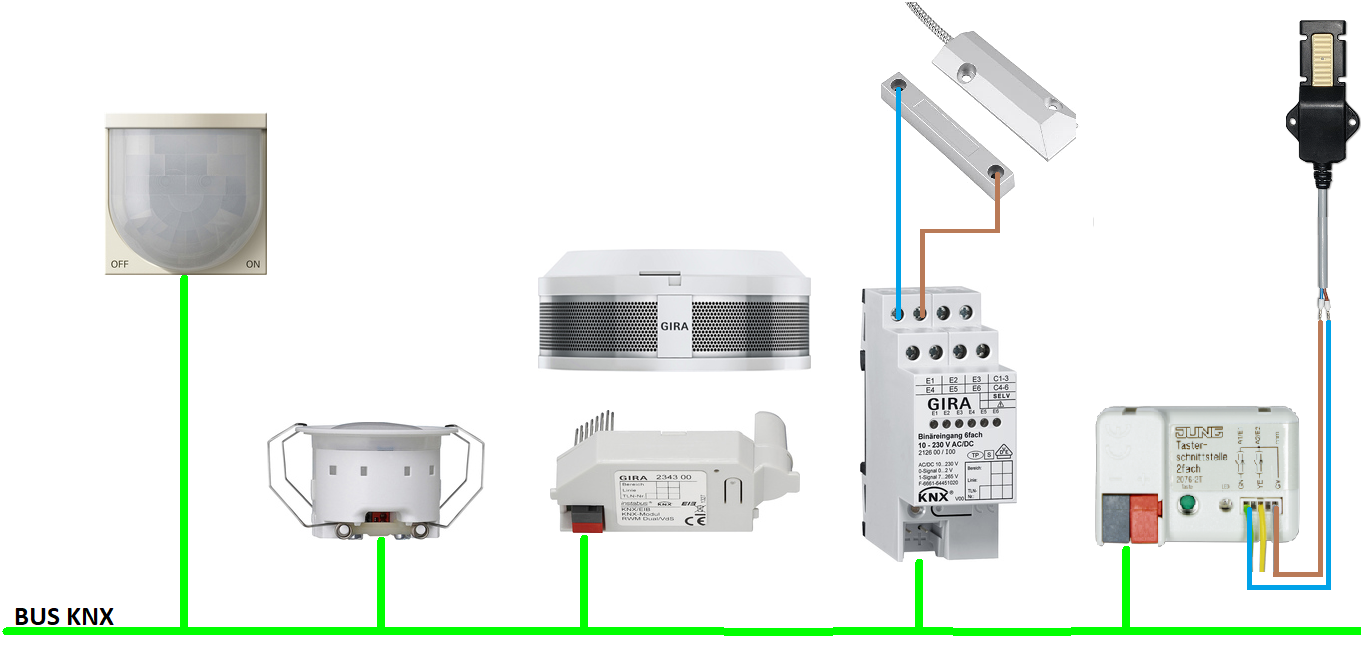
\includegraphics[width=1.15\textwidth]{figures/conex_sensores.png}   
\caption{Conexionado módulos sensoriales}
\label{fig:conex_sensores}
\end{figure}
\end{flushleft}